\documentclass[danish]{article}
\usepackage[utf8]{inputenc}
\usepackage[danish]{babel}
\usepackage[T1]{fontenc}	
\usepackage[a4paper, , margin=1in]{geometry}

\usepackage[version=3]{mhchem} % Package for chemical equation typesetting
\usepackage{siunitx} % Provides the \SI{}{} and \si{} command for typesetting SI units
\usepackage{graphicx} % Required for the inclusion of images
\usepackage{subcaption} % Add the possibility for subfigures/subcaptions.
\usepackage{natbib} % Required to change bibliography style to APA
\usepackage{amsmath} % Required for some math elements
\usepackage{gensymb}
\usepackage{float}
\graphicspath{ {graphics/} }
\setcounter{tocdepth}{1}
\setlength\parindent{0pt} % Removes all indentation from paragraphs

\renewcommand{\labelenumi}{\alph{enumi}.} % Make numbering in the enumerate environment by letter rather than number (e.g. section 6)
\begin{document}

\title{\textbf{ Introduktion til Reguleringsteknik }    Eksamensforberedelse}
\author{Jonas Lind}
\date{16-08-2017}
\maketitle
\tableofcontents
\newpage
\section{Øvelse 1 - Modellering af Blackbox}

\paragraph{Formål} med Øvelse 1 er at finde overføringsfunktionen for Blackbox med frekvenskarakteristikker og stepresonset.  Blackboxen skal repræsentere en ukendt "proces".
 
\paragraph{Forberedelse} for Øvelse 1 er forklaring af hvordan 1. og 2. ordenssystemer ser ud med et steprespons og deres reelle poler og komplekse poler. (side 3-4)
\begin{itemize}
	\item $\frac{1}{\alpha}$ = Tidskonstanten. Denne måles ved \SI{63}{\percent} af slutværdien.
	\item $T_r$ = Risetime, Denne måles fra \SI{10}{\percent} til \SI{90}{\percent}.
	\item $T_s$ = Setlingtime. Denne er når responset har nået \SI{98}{\percent} af den endelige værdi.
	\item Overføringsfunktionen $G(s)= \frac{K}{s+\alpha}$
\end{itemize}

Hvorledes bodeplot ser ud for 1. og 2. ordenssystemer. (side 5)
\begin{itemize}
	\item 1. ordens system har en pol der falder med $20 \si{\decibel}$ pr. dekade og har et fasedrej på \SI{45}{\degree} ved knækfrekvensen, \SI{3}{\decibel} frekvensen, \SI{90}{\degree} i alt. 
	\item 2. ordens system har to poler, hvor hver pol falder med $20 \si{\decibel}$ pr. dekade, \SI{40}{\decibel} i alt. Har et fasedrej på \SI{180}{\degree} i alt. 
\end{itemize}

Bestemme systemes stationære fejl overfor step- og rampe input. (side 6)
\begin{itemize}
	\item Stationær fejl ved stepinput $K_p = \lim\limits_{s\rightarrow 0} \dfrac{5000}{(s+50)(s+1000)}=1$
	\begin{itemize}
		\item $e(\infty)=\dfrac{1}{1+K_p} = \dfrac{1}{2}$
	\end{itemize}
	\item Stationær fejl ved rampeinput $K_v = \lim\limits_{s\rightarrow 0} s \dfrac{5000}{(s+50)(s+1000)}=0$
	\begin{itemize}
		\item $e(\infty)=\dfrac{1}{K_v} = \infty$
	\end{itemize}
\end{itemize}

Udformning af G1 så statinære fejl reduceres. 
\begin{itemize}
	\item Større forstærkning $K_p$.
	\item Tilføj et integrationsled $\frac{1}{s}$ på step og to integrationsled $\frac{1}{s^2}$ på rampe.
\end{itemize}

\paragraph{Praktisk} for Øvelse 1 er identificering af G(s) ud fra stepresponset. (side 8)

\begin{itemize}
	\item \si{\tau} \SI{19,2}{\milli\second}
	\item $\alpha = \frac{1}{\tau} = 52$
	\item $G(s)= \dfrac{\alpha}{s+\alpha} = \dfrac{52}{s+52}$
\end{itemize}

Identificere G(s) ud fra målepunkter og indsætte asymptoter. (side 10-11)
\begin{itemize}
	\item Lave et frekvenssweep og aflæse frekvens, amplitude og fase.
	\item Tegne \SI{20}{\decibel} pr. dekade og \SI{40}{\decibel} pr. dekade asymptotet på bodeplot og derved se overføringsfunktion G(s).
	\begin{itemize}
		\item Knækfrekvensen findes til at være ved \SI{9}{\hertz} og giver en pol ved $\SI{8}{\hertz}\cdot 2\pi \approx 56$.
		\item Ved ca. \SI{230}{\hertz} ses grafen falde \SI{40}{\decibel} pr. dekade kan endnu en pol findes ved $\SI{230}{\hertz}\cdot 2\pi \approx 1445$.
	\end{itemize}
\end{itemize}

Måling af stationære fejl, $V_{out} - V_{in}$. (side 12)
\begin{itemize}
	\item $K_p$ findes og derved kan den stationære fejl beregnes $K_p = A_{in}-A_{out} = 1 - 0,51 = 0,49$
	\begin{itemize}
		\item $ e(\infty)= \frac{1}{1+K_p} = \frac{1}{1+1} = 0,5$
	\end{itemize}
\end{itemize}


\section{Øvelse 2 -	Modulering af DC-motorstand}
\paragraph{Formål} med Øvelse 2 at bestemme overføringsfunktionen af motoren ud fra blokdiagram og databladet. Ved et steprespons bestemmes den faktiske overføringsfunktion af hele motorstanden.

\paragraph{Forberedelse} for Øvelse 2 er at bestemme overføringsfunktionen af motoren ud fra blokdiagrams manipulation. Blokdiagrammets parametre i SI-enheder findes i motorens datablad. 
\begin{itemize}
	\item Formel og blokdiagrammet over motor er udleveret.
	\item Bestemmelse af overføringsfunktionen ud fra blokdiagrammet. (side 4-5)
\end{itemize}

\begin{figure} [H]
	\centering
	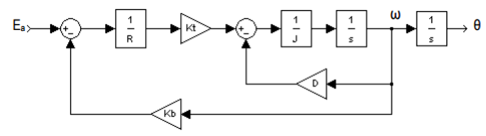
\includegraphics[width=0.6\linewidth]{graphics/ovelse2_1}
	\caption{Blokdiagram for motorstanden.}
	\label{fig:ovelse2_1}
\end{figure}

\begin{equation}
G_{\omega}(s) = \dfrac{\omega(s)}{E_a(s)} = \dfrac{K_t}{D R+K_b K_t+J R s}
\end{equation}

\begin{equation}
G_{\theta}(s) = \dfrac{\theta(s)}{E_a(s)} = \dfrac{K_t}{s(D R+K_b K_t+J R s)}
\end{equation}\\

Bestemmelse af parametre i SI-enheder ud fra databladet. (side 6)
\begin{itemize}
	\item $K_b$ = proportional faktor = (modinduceret spænding) \si{\volt\second\per\radian} (volt-seconds/radian)
	\item $R$ = ankermodstand = \SI{17,73}{\ohm}
	\item $K_t = K_b$ = proportional faktor =  drejningsmoment = \SI{43,9}{\milli\newton\per\ampere} (newton-meters/ampere)
	\item $J$ = inertimoment = \SI{10,5}{\gram\square\centi\meter}
	\item $D$ = væskefriktionskoefficienten
\end{itemize}

De to stationære ligninger bruges til at bestemme væskefriktionskoefficienten $D$ (side 6).
\begin{itemize}
	\item  $E_a = R_a I_a + K_b \omega$ 
	\item $T_m = K_t I_a = D \omega$ 	
\end{itemize}

\begin{equation}
D = \dfrac{T_m}{\omega} = 1,16\cdot 10^{-6} \si{\newton\meter}\frac{\si{\second}}{\si{\radian}}
\end{equation}\\

Ved at indsætte værdier i overføringsfunktionen $G_\omega(s)$ vises at $G_\omega(s) \approx \frac{2358}{s+105}$. (side 6)\\

Værdierne i $G_\omega(s)$ findes ud fra et stepresponse. 
\begin{itemize}
	\item $\alpha$ findes ved at måle tidskonstanten på et steprespons $\alpha = \frac{1}{\tau}$
	\item  Forstærkningen K findes ved at måle DC forstærkningen $K_{DC} = \frac{|V_{in}|}{|V_{out}|}$
\end{itemize}
\newpage
Belastning med anden inertimoment og væskefriktion. (side 7)
\begin{itemize}
	\item $D = D_a + D_b(\frac{N_1}{N_2})^2$
	\item $J = J_a + J_b(\frac{N_1}{N_2})^2$
\end{itemize}

\begin{figure} [H]
	\centering
	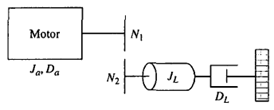
\includegraphics[width=0.35\linewidth]{graphics/ovelse2_2}
	\caption{Gearing.}
	\label{fig:ovelse2_2}
\end{figure}

Ændring af blokdiagram så $K_b$ tages ud lige efter $K_t$-blokken. (side 7)\\

Ændring af blokdiagram, så $K_b$ går til miderste sumpunkt. (side 8)\\

Ændring af blokdiagram, så selvinduktion kommer med. (side 8)
\begin{itemize}
	\item Den samlede impedans = $R+L s$
\end{itemize}

\paragraph{Praktisk} for Øvelse 2 at identificere motorstandens parametre ved målinger.

Måling af motorens ankermodstand fastholdt i forskellige stillinger. (side 10)
\begin{itemize}
	\item Når motoren "kører" vil der være andre kræfter, som spiller ind, blandt andet spolevirkning i motoren.
\end{itemize}

Måling af langsomste omdrejningstal og beregning af hurtig omdrjeningstal. (side 9)
\begin{itemize}
	\item Måling af $\omega = 45 rpm = \dfrac{45}{\SI{60}{\second}} 2\pi 24 = \SI{113,09}{\radian\per\second}$
	\item Beregning af $\omega_{tacho} = \dfrac{\SI{0,56}{\volt}}{\frac{\SI{0,52}{\volt}}{1000\,rpm}}\dfrac{1000\,rpm}{\SI{60}{\second}}2\pi = \SI{112,78}{\radian\per\second}$
\end{itemize}

Bestemmelse af motorstandens overføringsfunktion ud fra stepresons. (side 10-11)
\begin{itemize}
	\item Bestem $K_{ms}$, $\alpha_{ms}$ og $\tau_{ms}$  for motorstanden. 
	\begin{itemize}
		\item DC-forstærkningen $K_{DC}$ findes ved $\frac{\omega}{E_a}=22,62$
	\item Hvorved motorstandskonstanten $K_{ms}$ nu kan findes $K_{DC}\cdot \alpha_{ms}=611,43$
	\item $G_{ms}(s) = \dfrac{K_{ms}}{s+a_{ms}} = \dfrac{611,42}{s+27,03}$
	\end{itemize}
\end{itemize}

Amplitude og fasekarakteristik ud fra -3dB punktet. (side 11-12)
\begin{itemize}
	\item \SI{3}{\decibel} amplituden findes ved $\frac{\SI{595}{\milli\volt}}{\sqrt{2}} = \SI{421}{\milli\volt}$
	\item \SI{3}{\decibel} frekvensen findes ud fra polen $\frac{\alpha_{ms}}{2\pi} = \SI{4,3}{\hertz}$
	\begin{itemize}
		\item Fasen ved \SI{3}{\decibel} frekvensen \SI{4,3}{\hertz}  findes til ca. \SI{48}{\degree}. 
		\item Fasen ved \SI{3}{\decibel} amplituden \SI{422}{\milli\volt} findes til ca. \SI{39}{\degree}.
	\end{itemize}
\end{itemize}

Steprespons direkte fra funktionsgenerator. (side 13)
\begin{itemize}
	\item Modstanden er nu ankermodstanden i serie med \SI{50}{\ohm} fra udgangen af funktionsgeneratoren. 
	\item Indgangssignal får ikke strøm nok da den begrænses.
\end{itemize}
\newpage
\section{Øvelse 3 - Optimering af Blackbox}
\paragraph{Formål} med Øvelse 3 er at opbygge et reguleringssystem, hvor Blackboxen indgår i en lukket sløjfe. Blackboxens model blev udmålt i Øvelse 1 til $G(s)=\frac{50000}{(s+50)(s+1000)}$. 

\paragraph{Forberedelse} for Øvelse 3 dimensioneres en P-, en PD- og en PI- regulator ud fra givne dynamiske og statiske systemkrav.\\
\newline Amplitude og fasekarakteristik over systemet (blackbox) afbildes. Bruges til dimensionering af de forskellige regulatorer. (side 2)\\

G(s) reguleres med en P-regulator $G_c(s) = K_p$ som giver et $\si{\percent}$OS på \SI{5}{\percent}. (side 3) 

\begin{itemize}
	\item Forskellige $K_p$ værdier blev prøvet og ved \SI{21}{\decibel} ($11gg$) blev $\si{\percent}$OS = \SI{5}{\percent}.
	\item Fra steprespons kunne den stationære fejl og $T_r$ aflæses. 
	\begin{itemize}
		\item $e(\infty) = 1-0,917 = 0,083$, $T_r = \SI{2,66}{\milli\second}$, $\si{\percent}$OS aflæst til \SI{5,52}{\percent}.
		\item På bodeplot fås værdierne $\omega_{\theta m} = \SI{491}{\radian\per\second}$ og $\theta_m = \SI{69,7}{\degree}$.
	\end{itemize}
\end{itemize}
\vspace{3mm}
Gentag samme procedure for \SI{5}{\percent} OS bare med \SI{30}{\percent} OS (side 4).
\begin{itemize}
	\item Forskellige $K_p$ værdier blev prøvet og ved \SI{32,5}{\decibel} ($42gg$) blev $\si{\percent}$OS = \SI{30}{\percent}.
	\item Fra steprespons kunne den stationære fejl og $T_r$ aflæses.	
\begin{itemize}
	\item $e(\infty) = 1-0,977 = 0,023$, $T_r = \SI{0,958}{\milli\second}$, $\si{\percent}$OS aflæst til \SI{30}{\percent}.
	\item På bodeplot fås værdierne $\omega_{\theta m} = \SI{1290}{\radian\per\second}$ og $\theta_m = \SI{40,1}{\degree}$.
\end{itemize}
\end{itemize}
\vspace{3mm}
Design en Lead-regulator der reducerer $\si{\percent}$OS til \SI{5}{\percent}, med båndbredde = \SI{1290}{\radian\per\second}. (side 5-6)
\begin{itemize}
	\item Design regulator ud fra arket Analysis- and Design Procedure.
	\item Hvor meget fasemarginen skal forøges for at opnå \SI{5}{\percent} OS.
	\item $\beta$ = afstanden mellem nulpunkt og pol, giver faseboblen.
	\item T = placering af faseboblen.
	\item Samlet forstærkning skal reguleres så processen og regulatoren har forstærkningen 1 = \SI{0}{\decibel}. Derved findes værdien for $K_c$.
	\item Den stationære fejl findes ud fra stepresponset.
	\begin{itemize}
		\item  $e(\infty) 1-0,964=0,036$, $T_r = \SI{1,06}{\milli\second}$, $\si{\percent}$OS aflæst til \SI{5,47}{\percent}
		\item På bodeplot fås værdierne$\omega_{\theta m} = \SI{1280}{\radian\per\second}$  og  $\theta_m = \SI{65,6}{\degree}$.
	\end{itemize}
	\item Fasemarginen er blevet forøget og
	DC-forstærkningen ikke er blevet forringet.
\end{itemize}
\vspace{3mm}
PI-regulator (lag) dimensioneres så stationære fejl fjernes, ud fra opgave (b). (side 7-8)
\begin{itemize}
	\item Den stationære fejl ønskes fjernet helt og derved må $\alpha$ være uendelig stor.
	\begin{itemize}
		\item Herved ændres overføringsfunktionen og kaldes nu for en integralregulator.
	\end{itemize} 
	\item Nulpunkt placeres 10 gange under fasemarginsfrekvensen $\theta_m$ for ikke at påvirke denne.
	\item Bodeplot af Lag-regulator viser en negativ fase på \SI{6}{\degree}.
	\begin{itemize}
		\item Fasemarginen bliver herved lidt anderledes end beregnet.
	\end{itemize}
	\item Lag regulatoren hæver DC forstærkningen og formindsker den stationære fejl.
	\item Fasemarginfrekvensen er den samme.
\end{itemize}

\newpage
\paragraph{Praktiske del} for Øvelse 3 er at anvende de regulatorer der blev designet i forberedelsen.\\
P-regulator
\begin{itemize}
	\item Justere forstærkningen $K_p$, vise værdier for error, $\si{\percent}$OS og risetime. (side 9)
	\begin{itemize}
		\item Større forstærkning = mindre error, større $\si{\percent}$OS og mindre risetime.
	\end{itemize}
	\item Indstil $K_p$ så der kommer \SI{5}{\percent} OS og bestem error og risetime. 
	\begin{itemize}
		\item $e(\infty) = 40,2-38,6 = \SI{1,6}{\milli\volt}$, $T_r = \SI{2,8}{\milli\second}$
	\end{itemize}
	\item Indstil $K_p$ så der kommer \SI{30}{\percent} OS og bestem error og risetime. (side 10)
	\begin{itemize}
		\item $e(\infty) = 39,0-38,2 = \SI{0,8}{\milli\volt}$, $T_r = \SI{900}{\micro\second}$
	\end{itemize}
\end{itemize}
\vspace{3mm}
PD-regulator
\begin{itemize}
	\item Brug værdier fra beregnet Lead-regulator og se om \SI{5}{\percent} OS holder. (side 11)
	\begin{itemize}
		\item Der måles \SI{18}{\percent} OS, anvendt forkert $K_p$.
	\end{itemize}
	\item Stationære fejl og risetime bestemmes. 
	\begin{itemize}
		\item $e(\infty) = 38,6-38,2 = \SI{0,4}{\milli\volt}$, $T_r = \SI{490}{\micro\second}$
	\end{itemize}
\end{itemize}
\vspace{3mm}
PI-regulator
\begin{itemize}
	\item Indstilling af $K_p$ så \SI{5}{\percent} OS. (side 12)
	\item PI-regulator indstilles så stationære fejl fjernes men med samme \SI{5}{\percent} OS.
	\begin{itemize}
		\item Fortsat en stationær fejl på \SI{1}{\milli\volt}.
	\end{itemize}
	\item Når nulpunktet flyttes tættere på fasemarginsfrekvensen og oversvinget bliver større.
	\begin{itemize}
		\item $T_I$ øges = den stationære fejl bliver forværret og settling time bliver kortere.
	\end{itemize} 
\end{itemize}
\vspace{3mm}
PID-regulator
\begin{itemize}
	\item PID-regulator eliminerer oversving og steady-state error. Desuden formindskes $T_r$. (side 13)
	\item Prøve sig frem med \SI{5}{\percent} OS og lille risetime. 
\begin{itemize}
	\item P bestemmer $T_r$. Hvis den øges så forbedres risetime.
	\item I fjerner steady-state-error, men forøger oversving.
 	\item D formindsker oversving.
\end{itemize}
\end{itemize}

\newpage
\section{Øvelse 4 - DC-motoren som positionsservo}
\paragraph{Formål} med Øvelse 4 er at opbygge et positions reguleringssystem (positionsservo). Ud fra nogle systemkrav dimensioneres en lead-regulator og virkningen af en P, PI og Lead regulator afprøves. I denne øvelse kobles potentiometeret til måling af vinkeldrejningen. En effektforstærker og en Control box bruges til at realisere regulator-parametrene.


\paragraph{Forberedelse} for Øvelse 4 er at dimensionere en Lead-regulator ud fra givne dynamiske og statiske systemkrav. Systemoversigt blev givet samt parametre for modellen og overføringsfunktion med værdier.

\vspace{3mm}
P-regulator
\begin{itemize}
	\item Største $K_c$ værdi findes med $\si{\percent}$OS < \SI{5}{\percent}. Observere $\si{\percent}$OS, setlingtime og error. (side 3)
	\begin{itemize}
		\item $K_c = 39$, \SI{4,69}{\percent} OS og setlingtime = \SI{253}{\milli\second}, den stationære fejl $e(\infty) = 0$.
	\end{itemize}
	\item Amplitude og fasekarakteristik ud fra $K_c$ værdi. Fasemargin og Fasemarginfrekvens findes. (side 4)
	\begin{itemize}
		\item $\omega_{\theta m} = \SI{15,4}{\radian\per\second}$  og  $\theta_m = \SI{65}{\degree}$.
	\end{itemize}
	\item Den stationære fejl beregnes med værdier fra a) når det er rampeinput. (side 4)
	\begin{itemize}
		\item $K_v = 16,95$ og $e(\infty) = \SI{23,6}{\milli\volt}$.
	\end{itemize}
	\item Simulering af step og ramperespons med og uden PI-regulator. (side 5)
\end{itemize}
\vspace{3mm}
PI regulator anvendes ikke længere, herefter øges forstærknignen $K_p$. 
\begin{itemize}
	\item $K_c$ = 90 gg. Lav bodeplot og steprespons. (side 6)
	\begin{itemize}
		\item Mindre fasemargin $\theta_m = \SI{48,4}{\degree}$, højere fasemarginsfrekvens $\omega_{\theta m} = \SI{29,3}{\radian\per\second}$, større $\si{\percent}$OS = \SI{19,7}{\percent} og større setlingtime.
	\end{itemize}
\end{itemize}
\vspace{3mm}
Lead-regulator
\begin{itemize}
	\item Dimensionering med $\si{\percent}$OS < \SI{5}{\percent} og fasemarginfrekvens $\omega_{\theta m} = \SI{29,3}{\radian\per\second}$ (side 8)
	\begin{itemize}
		\item Beregninger ud fra formler/kurver som beskrevet i Analysis and Design Procedure.
	\end{itemize}
	\item Dimensionering af PD regulator ud fra lead-regulator.
	\begin{itemize}
		\item Beregninger og overføringsfunktion for PD regulator.
	\end{itemize}
	\item Bodeplot for lead-regulatoren. (side 9)
	\begin{itemize}
		\item Fasemargin hævet med $\omega_{\theta m} \approx \SI{16}{\radian\per\second}$ og fasemarginfrekvens fortsat den samme.
	\end{itemize}
	\item Steprespons for lead-regulator. (side 10)
	\begin{itemize}
		\item Væstentlig mindre oversving med \SI{3,66}{\percent} OS og forbedret setlingtime.
	\end{itemize}
\end{itemize}

\paragraph{Praktisk} for Øvelse 4 er at tilslutte et 10-turns-potentiometer til vinkelmåling på motorakslen. Herefter anvendes de regulatorer der blev desgignet i forberedelsen.\\


Indstilling af Control box $K_p=1$ og vippekontakten til $x10$. (side 10)
\begin{itemize}
	\item Når gain sættes til x10 bliver motoren mere følsom, mindre statisk fejl.
	\item \SI{300}{\milli\volt}-\SI{500}{\milli\volt} nås allerede ved \SI{30}{\milli\volt}-\SI{50}{\milli\volt} og den reagerer derfor hurtigere.
\end{itemize}

\vspace{3mm}
P-regulator
\begin{itemize}
	\item Justering af $K_p$ så $\si{\percent}$OS < \SI{5}{\percent} og sammenlign med forberedelsens værdier. (side 11)
	\item Samme indstillinger for funktionsgenerator, men nu med trekantskurve. Sammenlign stationær fejl med forberedelsen (side 12)
\end{itemize}
\vspace{3mm}
PI-regulator
\begin{itemize}
	\item 	Indsættelse af PI regulator fra forberedelsen. Sammenlign den stationære fejl. (side 12)
	\begin{itemize}
		\item Den stationære fejl er blevet væsentlig formindsket, men der opstår et større $\si{\percent}$OS.
	\end{itemize}
	\item Med firkant ind, iagtag $\si{\percent}$OS og formindsk $T_i$ og iagtag igen $\si{\percent}$OS. (side 13)
	\begin{itemize}
		\item Mindre $T_i$ resulterer i et større $\si{\percent}$OS og større setlingtime.
	\end{itemize}
	\item Formindsk forstærkning og iagtag $\si{\percent}$OS (side 13)
	\begin{itemize}
		\item Mindre gain resulterer i en langsommere setlingtime og større $\si{\percent}$OS.
	\end{itemize}
\end{itemize}
\vspace{3mm}
PI-regulator anvendes ikke.
\begin{itemize}
	\item Forstærkning $K_{pa} = 90 gg$. Og kig $\si{\percent}$OS. (side 14)
	\begin{itemize}
		\item \SI{22,8}{\percent} OS
	\end{itemize}
\end{itemize}
Realisere den lead-regulator fra forberedelsen og sammenlig resultater. (side 14)
\begin{itemize}
	\item Forbedret lead-regulator med justerede værdier for $K_c$, $T_D$ og $T_L$.
\end{itemize}

\newpage
\section{Øvelse 5 - Blackbox med tidsforsinkelse og digital Lead regulator}
\paragraph{Formål} med Øvelse 5 er at opbygge et digitalt reguleringssystem, hvor Blackboxen indgår samt er der nu også sættes en tidsforsinkelse ind i åbensløjfen. Der ses på hvorledes tidsforsinkelser og valg af samplingfrekvens påvirker reguleringssystemer.

\paragraph{Forberedelse} for Øvelse 5 undersøges virkningen ved både den højest og lavest anbefalede samplingsfrekvens iflg. Åstrøm og Wittenmark. Herefter designes en analog lead-regulator  således, at der kompenseres for tidsforsinkelsen. Til sidst beregnes den digitale lead-regulator ved en bilineær transformation.\\

Udgangspunkt i den analoge proportionalregulator fra Øvelse 3, OS=\SI{30}{\percent}, $K_p = 42$, $\omega_{\theta m} = \SI{1300}{\radian\per\second}$.

\vspace{3mm}
Virkningen af den højest og lavest anbefalede samplingsfrekvens iflg. Åstrøm og Wittenmark. (side 3)
\begin{itemize}
	\item Udregning af højest og lavest samplingfrekvens $\frac{0.15}{\omega_{\theta m}} \leq T \leq\frac{0.5}{\omega_{\theta m}}$.
	\begin{itemize}
		\item Sample intervallet T medfører en forsinkelse af signalet på $\frac{T}{2}$.
	\end{itemize}
	\item Bodeplot og steprespons.
	\item Fasemarginen er mindre ved den lave samplingsfrekvens i forhold til den høje samplingsfrekvens.
\end{itemize}
\vspace{3mm}
Indsættelse af tidsforsinkelse = 0.8 ms. (side 4-5)
\begin{itemize}
	\item Beregning af fasebidrag.
	\item Forventet reaktion af systemet.
\end{itemize}
\vspace{3mm}
Design analog lead-regulator der kompenserer for tidsforsinkelse. (side 5-6)
\begin{itemize}
	\item Beregninger via Analysis and Design Procedure.
	\item Tidsforsinkelsen er ikke medtaget for lead-regulatoren da den ikke bidrager med forstærkning.
	\item Fasemargin hævet til $\theta_m = \SI{40,5}{\degree}$.
\end{itemize}
\vspace{3mm}
Beregning af digital lead-regulator. (side 8-9)
\begin{itemize}
	\item Størst anbefalede og 10 gange mindre. 
	\item Bestemmelse af overføringsfunktion $G_0(z)$ samt beregning af overføringsfunktionerne. 
	\item Steprespons for begge samplingsfrekvenser.
\end{itemize}
\vspace{3mm}
\paragraph{Praktisk} for Øvelse 5 med samme opstilling af systemet som i Øvelse 3. Dog er der tilføjet en PSoC der udgør den digitale regulator og "Processens" tidsforsinkelse, $T_D$.
\begin{itemize}
	\item Højeste og laveste sample frekvens indflydelse på systemet. (side 11)
	\begin{itemize}
		\item  Ved laveste samplefrekvens fås $\si{\percent}$OS = \SI{68}{\percent} 
		\item Ved højeste samplefrekvens fås $\si{\percent}$OS = \SI{48}{\percent}.
	\end{itemize}
	\item Indflydelse af tidsforsinkelse på processen. (side 12)
	\begin{itemize}
		\item Systemet bliver ustabilt ved $K_p = 42$.
		\item Forstærkningen sæmkes indtil systemet er netop stabilt, $K_p \approx 32$, ca. \SI{150}{\hertz}.
		\item Systemet bliver ustabilt ved 
		$\omega_{\theta m} = \SI{1300}{\radian\per\second}$.
		\item Den målte frekvens hvor systemet begynder at oscillere er lidt under fasemarginfrekvensen $\omega = \SI{150}{\hertz}\cdot 2\pi \approx \SI{950}{\radian\per\second}$.
	\end{itemize}
	\item Virkningen af den digitale lead-regulator ved steprespons. (side 14)
	\begin{itemize}
		\item Den lave samplingfrekvens benyttes, da forstærkningen ikke kan realiseres på udstyret.
		\item $\si{\percent}$OS ligger lavere end forberedelserne.
	\end{itemize}
\end{itemize}

\newpage
\section{Øvelse 6 - DC-motoren som positionsservo med digital Lag- regulator}
\paragraph{Formål} med Øvelse 6 er at opbygge et digitalt reguleringssystem, hvor motorstanden indgår samt er der nu også tilføjes en tidsforsinkelse. Der ses på hvorledes tidsforsinkelser og valg af samplingfrekvens påvirker reguleringssystemer.

\paragraph{Forberedelse} for Øvelse 6 undersøges virkningen ved både den højest og lavest anbefalede samplingsfrekvens iflg. Åstrøm og Wittenmark. Herefter undersøges lag-regulatorens forventede påvirkning af stationære- og dynamiske egenskaber. Til sidst beregnes den digitale lag-regulator ved en bilineær transformation.\\

Overføringsfunktion er givet og fasemargin og fasemarginfrekvens undersøges med matlab.

\vspace{3mm}
PSoC sættes ind efter controlbox og indvirkning af samplingsfrekvenser, Åstrøm og Wittenmark (side 3)
\begin{itemize}
	\item 	Udregning af højest og lavest samplingfrekvens $\frac{0.15}{\omega_{\theta m}} \leq T \leq\frac{0.5}{\omega_{\theta m}}$.
	\begin{itemize}
		\item Sample intervallet T medfører en forsinkelse af signalet på $\frac{T}{2}$.
	\end{itemize}
	\item Bodeplot og steprespons.
	\item Fasemarginen er mindre ved den lave samplingsfrekvens i forhold til den høje samplingsfrekvens.
\end{itemize}
\vspace{3mm}
Indsættelse af tidsforsinkelse og beregning af fasebidrag. (side 5)
\begin{itemize}
	\item Fasebidraget er lille da systemet har lille båndbredde, $\theta_m = \SI{0,69}{\degree}$.
	\item Derfor ingen grund til at medregne tidsforsinkelse.
\end{itemize}
\vspace{3mm}
Indsættelse af lag-regulator og dens påvirkning på systemet. (side 6)
\begin{itemize}
	\item Overføringsfunktion givet.
	\item Regulator ikke designet rigtigt da faseboble er 5 gange under fasemarginsfrekvensen.
	\begin{itemize}
		\item Anbefaling er 10 gange under fasemarginfrekvensen.
		\item Giver et større negativt fasebidrag, $\theta_m \approx \SI{9}{\degree}$.
	\end{itemize}
\end{itemize}
\vspace{3mm}
Simulering med ramperespons med højst anebefalede samplingsfrekvens (side 7-8)
\begin{itemize}
	\item Er et type 1 system så ved steprespons vil fejl = 0.
	\item Beregning af den stationære fejl teoretisk og sammenligning med simuleringen.
	\begin{itemize}
		\item $K_v =\lim_{s\rightarrow 0}(s\cdot G_c(s)\cdot G(s))$
	\end{itemize}
\end{itemize}

\paragraph{Praktisk} for Øvelse 6 er at se påvirkningen af tidsforsinkelsen ved højeste og laveste samplingsfrekvens. 

\vspace{3mm}
System koblet op som analog, uden PSoC og kontrol af $\si{\percent}$OS < \SI{5}{\percent}. (side 9)

\vspace{3mm}
Indflydelse af samplingsfrekvenser på systemet. (side 9-10)
\begin{itemize}
	\item Større samplingsfrekvens = mindre $\si{\percent}$OS.
\end{itemize}
\vspace{3mm}
Digitale lag-regulator indsat, med rampeinput. (side 10-11)
\begin{itemize}
	\item De stationære egenskaber er væsentligt forbedret med lag-regulatoren.
	\begin{itemize}
		\item Mindre stationær fejl, medfører lidt større oversving.
	\end{itemize}
\end{itemize}

\end{document}
